% GENERATED FILE -- do not edit by hand.
% Source: output\runs\sled-coi-reduction-v1\result.json
% SHA-256: 8f5ab582212da4ad95e08c3ce0c32b9ce1e36fce808df813ada6008b6ae9e1ca
% Run: python scripts/generate_paper_figures.py

\begin{figure}[t]
\centering
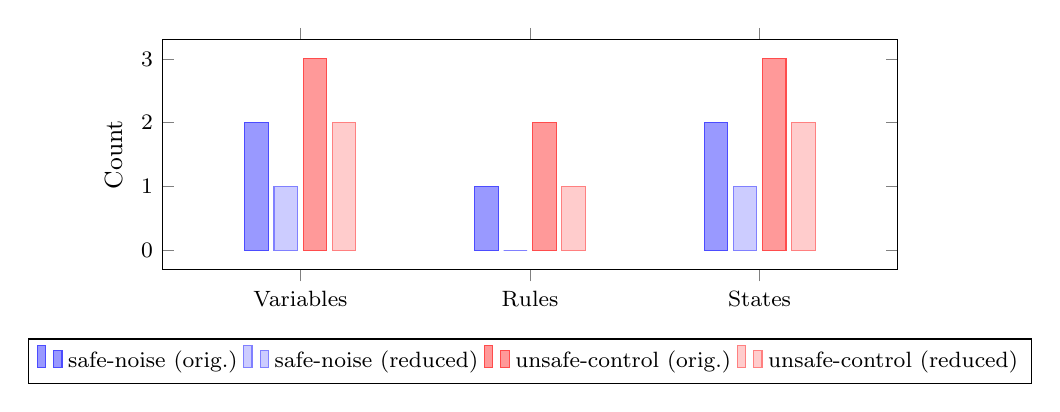
\begin{tikzpicture}
\begin{axis}[
    width=0.9\columnwidth,
    height=4.5cm,
    ybar,
    bar width=0.3cm,
    enlarge x limits=0.3,
    ylabel={Count},
    ylabel style={font=\small},
    symbolic x coords={Variables, Rules, States},
    xtick=data,
    x tick label style={font=\footnotesize},
    yticklabel style={font=\footnotesize},
    legend style={at={(0.5,-0.3)}, anchor=north, legend columns=4, font=\footnotesize},
]
\addplot[fill=blue!40, draw=blue!70] coordinates {
    (Variables, 2) (Rules, 1) (States, 2)
};
\addplot[fill=blue!20, draw=blue!50] coordinates {
    (Variables, 1) (Rules, 0) (States, 1)
};
\addplot[fill=red!40, draw=red!70] coordinates {
    (Variables, 3) (Rules, 2) (States, 3)
};
\addplot[fill=red!20, draw=red!50] coordinates {
    (Variables, 2) (Rules, 1) (States, 2)
};
\legend{safe-noise (orig.), safe-noise (reduced), unsafe-control (orig.), unsafe-control (reduced)}
\end{axis}
\end{tikzpicture}

\vspace{2mm}
\small
\begin{tabular}{lccccc}
\toprule
Fixture & Variables & Rules & States & Verdict (orig/red) & Agree \\
\midrule
safe-noise & 2 $\to$ 1 & 1 $\to$ 0 & 2 $\to$ 1 & safe / safe & True \\
unsafe-control & 3 $\to$ 2 & 2 $\to$ 1 & 3 $\to$ 2 & unsafe / unsafe & True \\
\bottomrule
\end{tabular}
\caption{Cone-of-influence reduction on two finite IR fixtures.
Reduction removes the noise variable and its associated rules in both
cases; verdicts agree between original and reduced models.  The unsafe
witness lifts to the original model.}
\label{fig:coi-reduction}
\end{figure}
